%\documentclass[aps,prb,a4paper,10pt,twocolumn,showpacs,floatfix,superscriptaddress,amsmath,amsfonts,amssymb,preprintnumbers]{revtex4-1}
\documentclass[aps,prb,a4paper,10pt,twocolumn,showpacs,floatfix,superscriptaddress,preprintnumbers,longbibliography]{revtex4-2}
\setlength\topmargin{-64pt}
\setlength\textheight{741pt}


%\usepackage{silence}
%\WarningFilter{revtex4-2}{Repair the float}
% To silence innocuous revtex warning!

% To clean up the bibliography entries and export only the relevant ones, use:
% bibclean messy_ini.bib > long_nice.bib
% bibexport -o minimal.bib manuscript.aux

%\usepackage[T1]{fontenc}
%\usepackage[utf8]{inputenc}
\usepackage{float}
\usepackage{dcolumn,graphicx,color,booktabs,microtype,afterpage}
\usepackage{amssymb}
\usepackage{amsmath}
\usepackage[charter,greekuppercase=italicized]{mathdesign}
\usepackage{sidecap}
\usepackage[mathlines]{lineno}

\graphicspath{{./}{figure/}}
\renewcommand{\tablename}{Table}
\makeatletter\renewcommand{\fnum@figure}[1]{\figurename~\thefigure.~}\makeatother
\makeatletter\renewcommand{\fnum@table}[1]{\tablename~\thetable.}\makeatother

\newcount\hh \newcount\mm
\hh=\time \divide\hh by 60
\mm=\hh \multiply\mm by 60 \mm=-\mm
\advance\mm by \time
\def\now{\number\hh:\ifnum\mm<10{}0\fi\number\mm}

\usepackage[colorlinks,plainpages=false,linkcolor=blue,urlcolor=blue,citecolor=blue,pdfpagemode=UseNone,pdfstartview=FitBH]{hyperref}
%\usepackage{nicefrac}

\newcommand{\half}{\frac{1}{\protect\raisebox{0.8pt}{\scriptsize 2}}}
\newcommand{\threehalf}{\frac{3}{\protect\raisebox{0.8pt}{\scriptsize 2}}}
\newcommand{\unsim}{\mathord{\sim}}

\newcommand{\tcr}[1]{\textcolor{black}{#1}}
\newcommand{\tcb}[1]{\textcolor{blue}{#1}}
\newcommand{\comm}[1]{\textcolor{green}{#1}}

\newcommand{\tabincell}[2]{\begin{tabular}{@{}#1@{}}#2\end{tabular}}

\hyphenation{non-centro-sym-met-ric centro-sym-met-ric iso-struc-tur-al su-per-flu-id}

%\synctex=1  % Enable/disable inverse search: pdf -> tex


\begin{document}

\makeatletter\renewcommand{\ps@plain}{%
\def\@evenhead{\hfill\itshape\rightmark}%
\def\@oddhead{\itshape\leftmark\hfill}%
\renewcommand{\@evenfoot}{\hfill\small{--~\thepage~--}\hfill}%
\renewcommand{\@oddfoot}{\hfill\small{--~\thepage~--}\hfill}%
}\makeatother\pagestyle{plain}

\preprint{\textit{Preprint: \today, \now.}} %For internal use only, do not distribute.}}
%\linenumbers

\title{Unusual $^{27}$Al NMR shift in the Weyl-fermion systems LaAlGe and PrAlGe}
%
\author{D.\ Tay}\email[Corresponding author:\\]{danieltay@phys.ethz.ch}
\affiliation{Laboratorium f\"ur Festk\"orperphysik, ETH Z\"urich, CH-8093 Zurich, Switzerland}
%
\author{T.\ Shang}
\affiliation{Key Laboratory of Polar Materials and Devices (MOE), School of Physics 
and Electronic Science, East China Normal University, Shanghai 200241, China}
\affiliation{Laboratory for Multiscale Materials Experiments, Paul Scherrer Institut, Villigen CH-5232, Switzerland}
%
\author{P.\ Puphal}
\affiliation{Laboratory for Multiscale Materials Experiments, Paul Scherrer Institut, Villigen CH-5232, Switzerland}
\affiliation{Max-Planck Institute for Solid State Research, D-70569 Stuttgart, Germany}
%
\author{E.\ Pomjakushina}
\affiliation{Laboratory for Multiscale Materials Experiments, Paul Scherrer Institut, Villigen CH-5232, Switzerland}
%
\author{H.-R.\ Ott}
\affiliation{Laboratorium f\"ur Festk\"orperphysik, ETH Z\"urich, CH-8093 Zurich, Switzerland}
\affiliation{Paul Scherrer Institut, CH-5232 Villigen PSI, Switzerland}
%
\author{T.\ Shiroka}\email[Corresponding author:\\]{tshiroka@phys.ethz.ch}
\affiliation{Laboratorium f\"ur Festk\"orperphysik, ETH Z\"urich, CH-8093 Zurich, Switzerland}
\affiliation{Paul Scherrer Institut, CH-5232 Villigen PSI, Switzerland}
%
%
%\affiliation{Paul Scherrer Institut, CH-5232 Villigen PSI, Switzerland}



\begin{abstract}
\noindent
LaAlGe and PrAlGe are members of the $R$AlGe series of compounds
(with $R$ a light rare-earth element), which have been shown to
host Weyl fermions. By exchanging the rare-earth cation, $R$AlGe
offers a remarkable tunability of its electronic properties, thereby
allowing to identify the electronic response of Weyl semimetals under
varying temperature- and magnetic-field conditions. 
%
Through a comparative $^{27}$Al NMR study of LaAlGe and PrAlGe, we
show that the rare-earth element can also be used to tune the NMR
response of Weyl fermions in the host. In both cases, we observe
unusual NMR shifts that deviate significantly from those
in ordinary metals such as Al. In LaAlGe, we report the observation
of a small negative shift, strongly varying with temperature, %but consistent
which can be explained by a recent theory of NMR shifts invoking Weyl
fermions. In PrAlGe, instead, we report a giant positive
NMR shift, of up to 20\% at 6\,K, most likely due to the transferred
hyperfine field from the Pr$^{3+}$ 4$f$-electron local moments. We
discuss the implications of our findings on future studies of 
Weyl-fermion systems. 
%
%Here, by a comparative $^{27}$Al NMR study of $R$AlGe, we show that the
%rare-earth element can also be used to tune the NMR response of Weyl
%fermions in the host. In both LaAlGe and PrAlGe, we observe 
%unusual NMR shifts that deviate significantly from %those %NMR shifts observed
%that in ordinary metallic Al. In LaAlGe, we report the observation
%of a small negative shift, consistent with the theory of NMR shifts for
%Weyl fermions. In PrAlGe, instead, we report %the observation of 
%a giant positive NMR shift, of up to 20\% at 6\,K, most likely due to 
%the transferred hyperfine field from the Pr$^{3+}$ 4$f$ electrons. 
%We suggest that, with a suitable choice of the rare-earth element, 
%$R$AlGe can serve as a platform for studying the interplay between 
%the transferred hyperfine fields and Weyl fermions.  
%
\end{abstract}

%\keywords{weyl semimetal, ferromagnetism, nuclear magnetic resonance}

\maketitle\enlargethispage{3pt}
 
%\section{Introduction}

%
\emph{Introduction.---} The $R$AlGe compounds (with $R$ a light rare-earth element, such as La, 
Ce, or Pr) have been shown to adopt a noncentrosymmetric LaPtSi-type 
crystal structure \cite{Gladyshevskii2000}, thus emerging % consequently are 
as good candidates for hosting Weyl nodes in their electronic excitation 
spectra \cite{Armitage2018}. Recent theoretical work \cite{chang2018magnetic} 
has established that also compounds with local moments on the rare-earth
sites (in this case Ce or Pr) still qualify as Weyl semimetals.
This is remarkable, since cations carrying magnetic moments generally
lead to complications at low temperatures, where magnetic ordering
breaks the time-reversal symmetry.
%also compounds with $R$ a light rare-earth metal 
%such as Ce or Pr would qualify as Weyl semimetals, in spite of the 
%cations carrying magnetic moments leading to complications at low 
%temperatures due to effects of ordered magnetic moments breaking time-reversal symmetry.
Results of subsequent ARPES experiments confirmed these theoretical
predictions in both LaAlGe \cite{xue2017discovery} and PrAlGe
\cite{sanchez2020observation}. 
In addition, results of measurements of the anomalous Hall- and Nernst 
effects \cite{destraz2020magnetism} provided indirect evidence of the 
Weyl nodes in PrAlGe, consistent with the theoretically calculated 
Berry curvature %in PrAlGe
\cite{destraz2020magnetism}. Hence, to date the existence of Weyl
nodes in the electronic excitation spectra of the $R$AlGe family
is well established.

The low-temperature magnetic properties of these compounds are
definitely more elusive, since they depend on the details of their
chemical composition and, indirectly, also on the synthesis
process \cite{puphal2019bulk}. 
Recent magnetotransport measurements on PrAlGe revealed that, 
instead of the simple ferromagnetic ground state predicted by theory
\cite{chang2018magnetic}, 
the magnetic phase diagram of PrAlGe is more complex than 
anticipated~\cite{destraz2020magnetism}. The present state of 
understanding of the interplay between local magnetic moments,
external magnetic fields, and Weyl nodes is thus incomplete.  

In this paper, we first compare the unusual temperature dependence
of the negative nuclear magnetic resonance (NMR) shift in the $^{27}$Al
NMR spectra of LaAlGe with that in an ordinary metal such as aluminum.
The data differ significantly from those reported previously in
Refs.~\cite{Wang2020landau} and \cite{antonenko2019nmr} for
other Weyl semimetals. In the first case, a positive shift of the
$^{75}$As resonance with a considerable temperature dependence was
noted in TaAs \cite{Wang2020landau}. In the second case, the $^{125}$Te
resonance line in WTe$_2$ revealed a negligible temperature dependence
of the shift and no information on the sign was provided %is available
\cite{antonenko2019nmr}.
The recorded shifts of up to 18\% we report here for the $^{27}$Al
resonance in PrAlGe are significantly larger in magnitude, again
exhibiting a considerable temperature dependence. Both features
are most likely due to the influence of the transferred hyperfine fields
caused by the interplay between the local Pr$^{3+}$ 
$4f^2$ electronic moments
and the fermions in the vicinity of the Weyl nodes in the $R$AlGe series.


%In this paper, we report yet another unexpected feature: the observation 
%of a giant nuclear magnetic resonance (NMR) shift, of up to 20\%, in 
%the $^{27}$Al NMR spectra of PrAlGe.  
%This is many orders of magnitude larger than the NMR shifts observed in 
%many standard metallic alloys, as well as in other Weyl semimetal systems, 
%such as TaAs \cite{Wang2020landau} and WTe$_{2}$ \cite{antonenko2019nmr}.
%
%Such giant NMR shift is observed in PrAlGe only and, as we show below, 
%is absent in the nonmagnetic parent compound LaAlGe. Therefore, its 
%origin might reflect the interplay between the local ionic moments due 
%to the Pr$^{3+}$ $4f$ electrons and the Weyl nodes in the $R$AlGe family.

%\section{Methods}
%
\emph{Methods.---} First, PrAlGe polycrystalline rods for the
floating-zone growth were cast by induction melting of the three
starting elements Pr, Al, and Ge with a purity of 99.99\% or better in a
high-frequency ac electric field. %strongly changing magnetic field.
The melting was followed by a sudden switch-off of the field, causing 
the melt to drop into a cooled copper hearth. The rods were then 
transferred into a SCIDRE HKZ high-pressure, high-temperature, optical 
floating-zone furnace. Further details can be found in
Ref.~\cite{puphal2019bulk}.
%The floating-zone growth was performed in a 
%purified argon atmosphere with a pressure of 5\,bar and a flow of 
%0.1\,l/min. With a rotation speed of $\pm 0.25$\,Hz ($15$\,rpm) and a 
%growth rate of 12\,mm/h, two dominant grains developed after a few 
%millimeters of growth, %both with their $a$ axes along the growth direction. 
%whose $a$ axes coincide with the growth direction. 
%From the resulting boule,
An oriented crystal of approximately 50\,mg was finally cut for the
NMR experiments.
The LaAlGe polycrystalline sample was prepared by the arc-melting method.
In both cases, phase purity was checked via x-ray diffraction using a
D8 Advance Bruker diffractometer with Cu K$\alpha$ radiation.
%Additional details on the growth method and the complete characterization
%dataset can be found in Ref.~\cite{puphal2019bulk}.

The magnetic susceptibility data shown below were re\-cord\-ed by means 
of a Quantum Design magnetic property mea\-sure\-ment system. %(MPMS). 
%Since the susceptibility is known to saturate at high fields \cite{puphal2019bulk}, 
%the Clogston-Jaccarino plot of the susceptibility vs NMR shift show 
%the susceptibility data acquired at 0.1\,T vs the NMR shifts measured at 5 and 7\,T.
%
The NMR spectra were collected in a temperature range between 5 and 300\,K 
via the spin-echo method by using $\pi/2$--$\pi$ rf pulses of 5 and 
10\,$\mu$s, respectively, with typical delays between the pulses of 
20\,$\mu$s. %by employing a fast Fourier transform (FFT) of the 
The $^{27}$Al NMR reference signal was obtained by measuring the NMR 
resonance in metallic Al at room temperature and then by scaling its 
frequency to that of 1.1\,m Al(NO$_{3}$)$_{3}$ in D$_{2}$O.
%



%\section{Experimental results}
%
\begin{figure*}[!bht]
	\centering 
	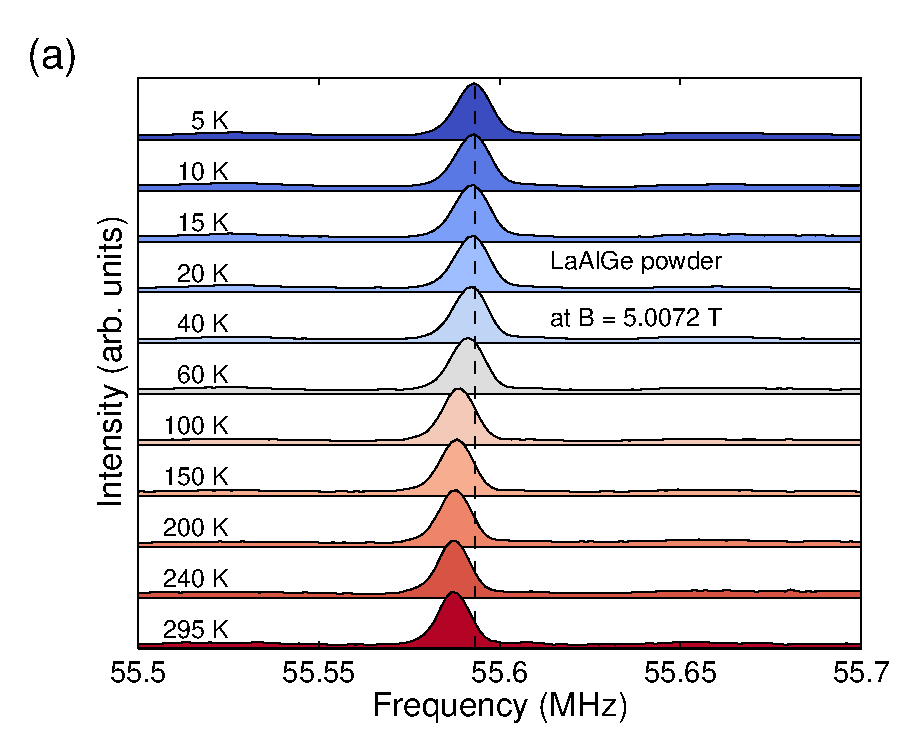
\includegraphics[width=0.32\textwidth,angle=0]{figures/LaAlGe_Powder/LaAlGe_powder_lines_vs_temp} 
	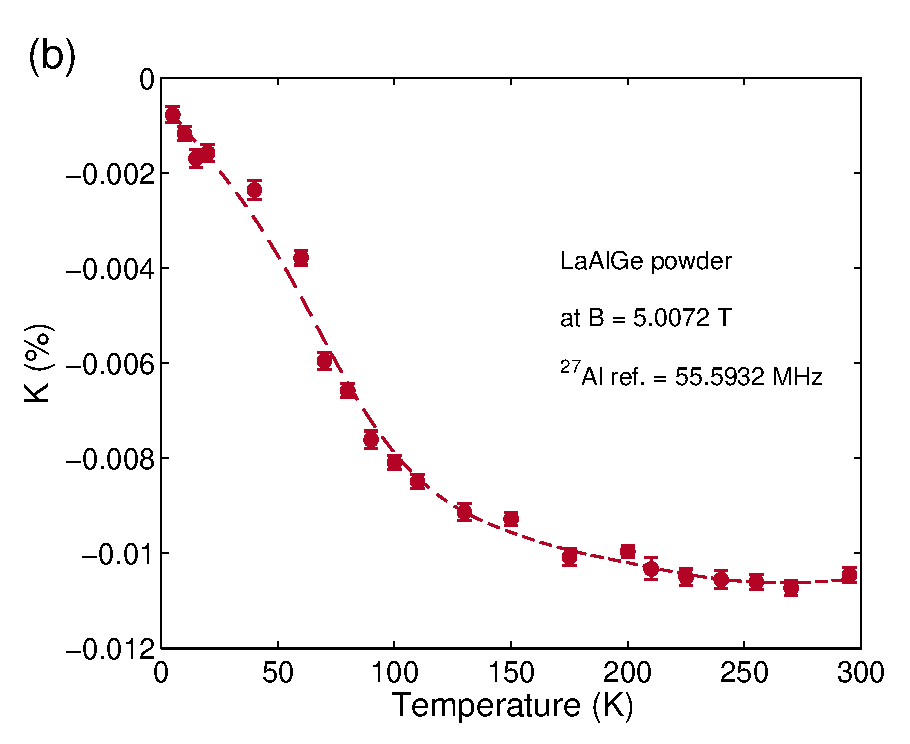
\includegraphics[width=0.32\textwidth]{figures/LaAlGe_Powder/gaussianshiftperc}%\label{fig:LaAlGe_shifts}}
	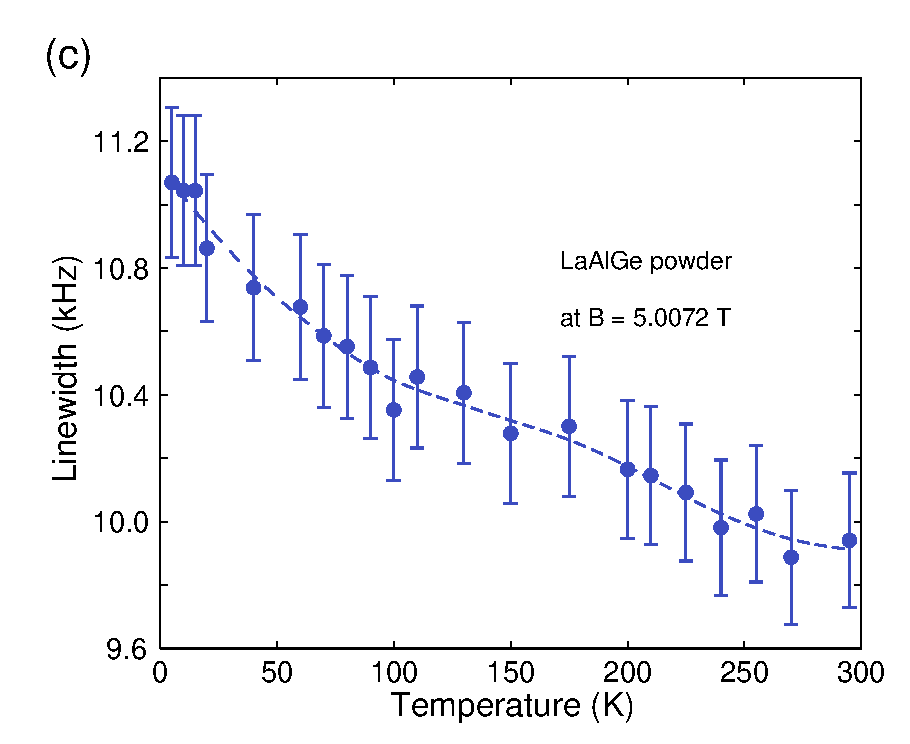
\includegraphics[width=0.32\textwidth]{figures/LaAlGe_Powder/gaussianwidth}%\label{fig:LaAlGe_widths}
	\caption{\label{fig:LaAlGe}(a) Line shapes, (b) line shifts,  and (c) line widths of $^{27}$Al 
	NMR in nonmagnetic LaAlGe powder, measured in a 5-T applied magnetic field. 
	The vertical line in (a) indicates the position of the reference Al NMR signal, %-- 1.1 m Al(NO$_{3}$)$_{3}$ in D$_{2}$O 
	while the dashed line in (b) is a fit to Eq.~\eqref{eqn:knightshiftmasterequation} 
	and a guide to the eyes in (c). As shown in panels (b) and (c), 
	in the nonmagnetic La case, neither the line shifts nor widths exceed 
	a few hundredths of a percent. Note that the $^{27}$Al line in Al metal
	is practically temperature independent and located at +0.16\% \cite{Knight1949}.} % [see also Fig.~\ref{fig:weylKS}(b)].}
\end{figure*}
%
% Relative to AlCl3 solution the Knight shift at 298 K was found to be 1640 +/- 1 ppm.
% More precise determination of the Knight shift of aluminium
% E.R.Andrew, W.S.Hinshaw, R.S.Tiffen
% Physics Letters A, Vol. 46, Issue 1, 19 November 1973, Pages 57--58.


%
\begin{figure*}[!htb]
	\centering 
	%% 5 T top
	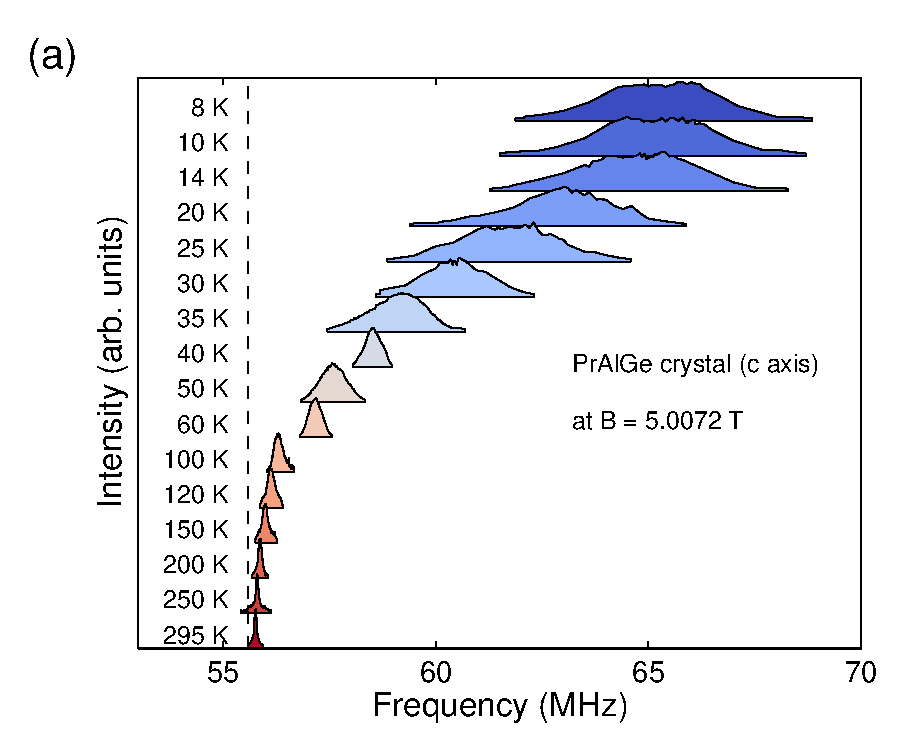
\includegraphics[width=0.32\textwidth,angle=0]{figures/PrAlGe_c_axis_5T/PrAlGe_c_axis_lines_vs_temp}%\label{fig:PrAlGe_c_axis_5T_lines}}
	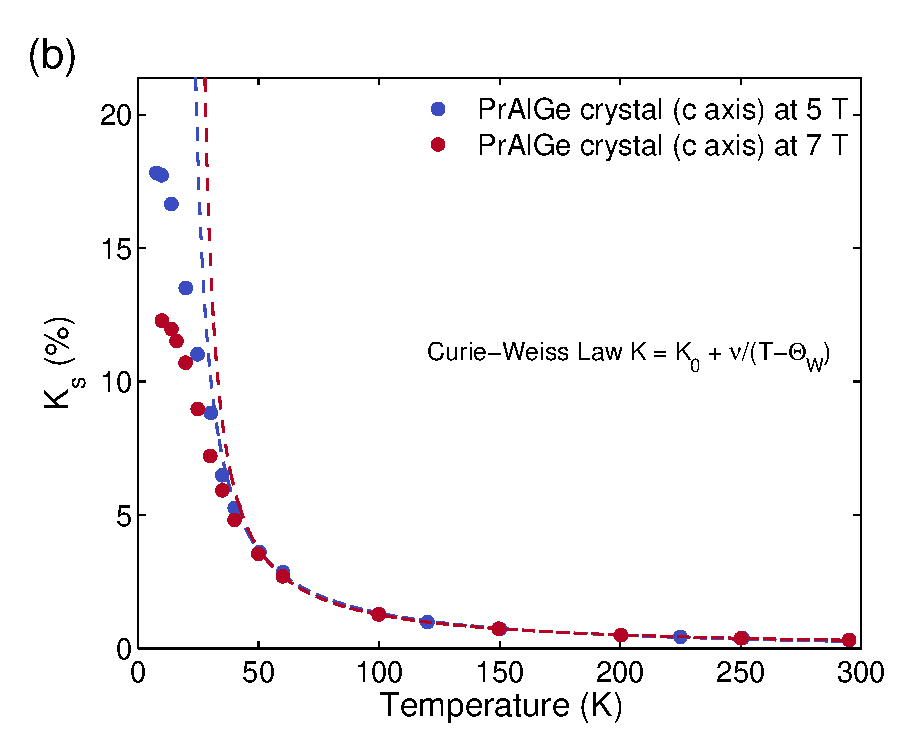
\includegraphics[width=0.32\textwidth]{figures/PrAlGe_c_axis_5T/27AlS_vs_T}%\label{fig:PrAlGe_c_axis_5T_shifts}
	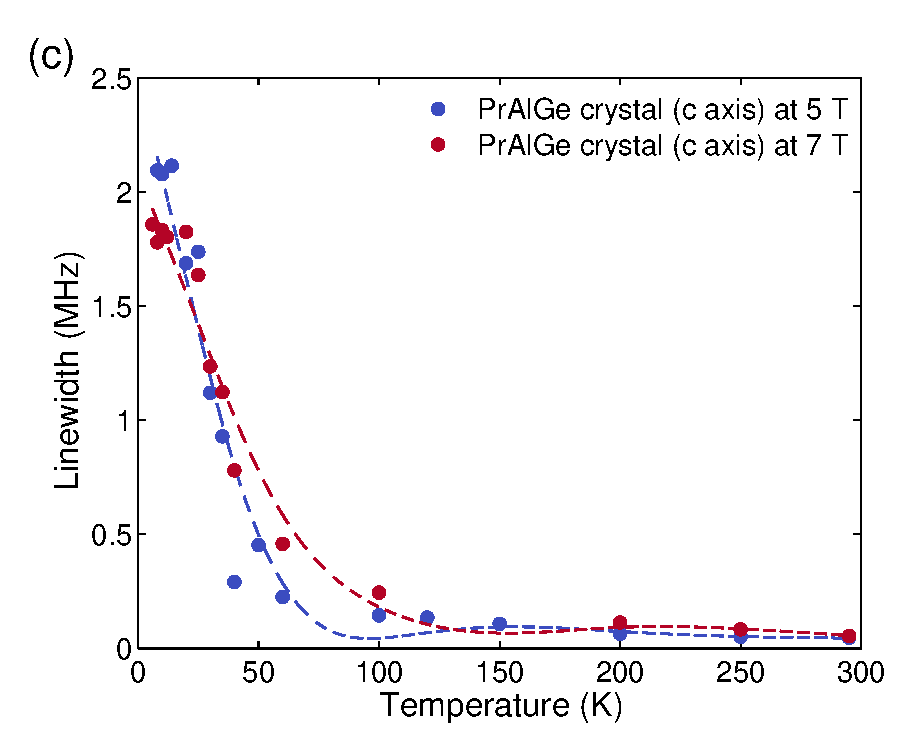
\includegraphics[width=0.32\textwidth]{figures/PrAlGe_c_axis_5T/27Alwidth_vs_T}%\\[5mm]%\label{fig:PrAlGe_c_axis_5T_widths}
	%% 7 T bottom	%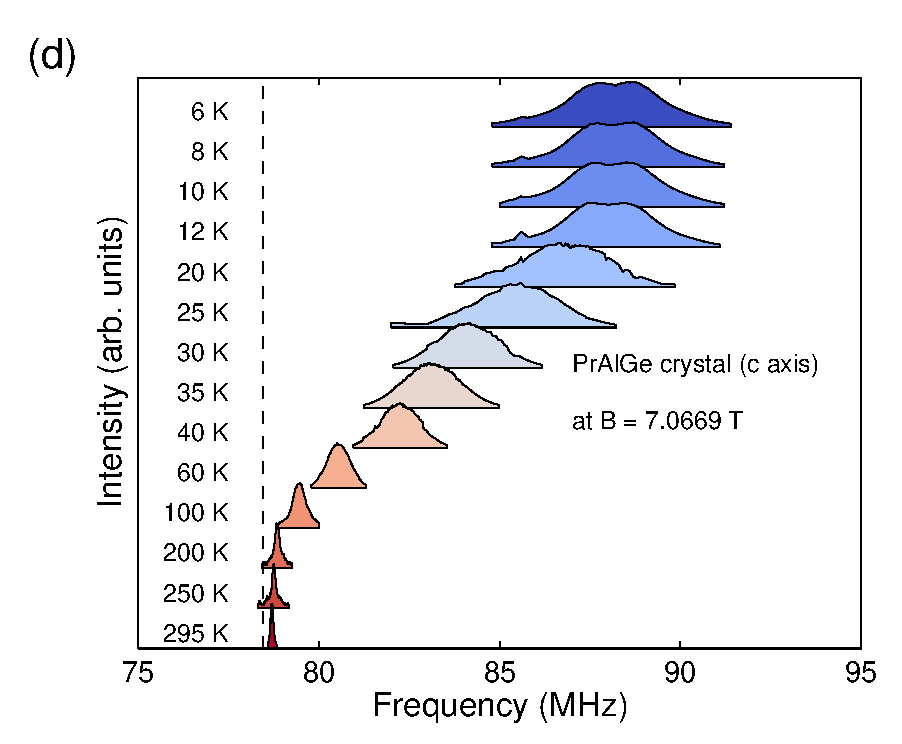
\includegraphics[width=0.32\textwidth,angle=0]{figures/PrAlGe_c_axis_7T/PrAlGe_c_axis_lines_vs_temp}%\label{fig:PrAlGe_c_axis_7T}  %\label{fig:PrAlGe_c_axis_7T_lines}	%%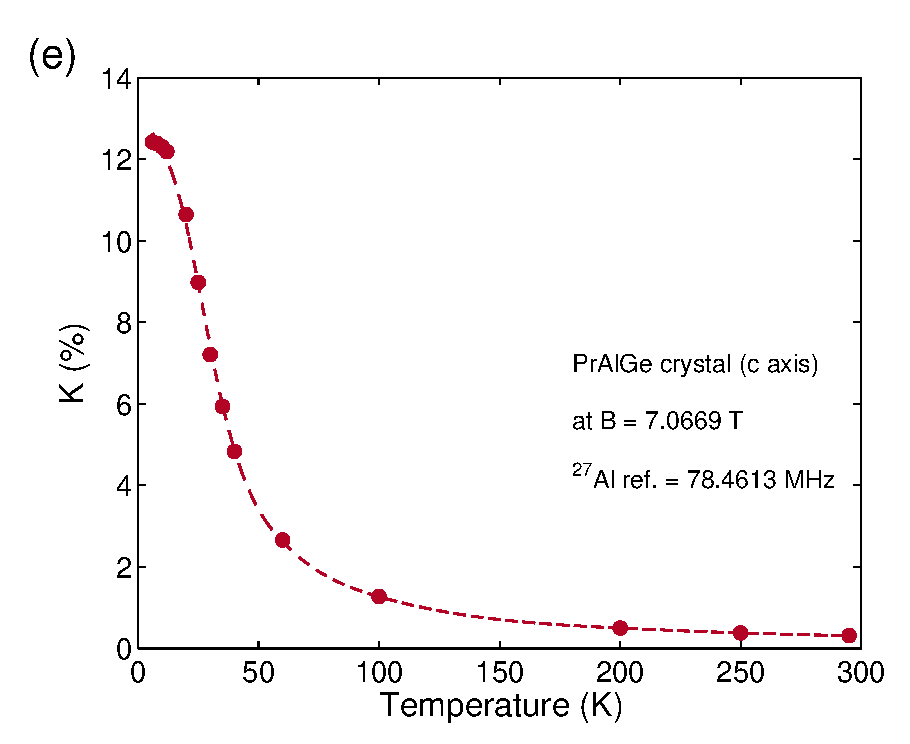
\includegraphics[width=0.32\textwidth]{figures/PrAlGe_c_axis_7T/gaussianshiftperc}%\label{fig:PrAlGe_c_axis_7T_shifts}	%%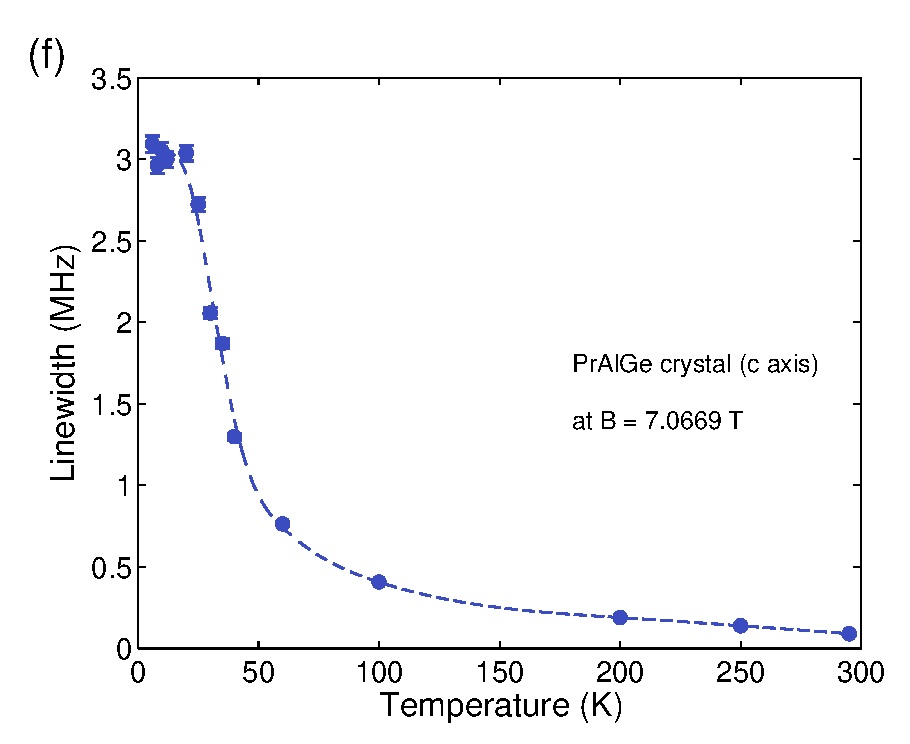
\includegraphics[width=0.32\textwidth]{figures/PrAlGe_c_axis_7T/gaussianwidth}%\label{fig:PrAlGe_c_axis_7T_widths}
	\caption{\label{fig:PrAlGe_c_axis_5T}(a) Line shapes, (b) line shifts,  and (c) line widths of $^{27}$Al NMR in a magnetic PrAlGe crystal aligned along the $c$-axis, measured in an externally applied field of 5 and 7\,T (the line shapes at 7\,T, not shown, are similar to those at 5\,T). 
	The vertical lines indicate the position of the reference Al NMR signal, while the dashed lines are fits or guides to the eye. Note the giant shift of the NMR lines in panel (b) and the significant line broadening below 100\,K in panel (c).}
\end{figure*}
%

\emph{Experimental results.---} First we consider the $^{27}$Al NMR
spectra of paramagnetic LaAlGe (with a closed $5p^6$ configuration, 
La$^{3+}$ has no magnetic moment). 
%https://www.webelements.com/lanthanum/atoms.html
Since $^{27}$Al is a spin-5/2 nucleus, ordinarily we expect to observe 
five NMR lines, reflecting the quadrupole interaction of the non-spherical 
nucleus with its electronic surroundings. 
It turns out that the quadrupole splitting is quite small and the 
satellite signals rather weak, such that they are not discernible in 
the spectra shown in Fig.~\ref{fig:LaAlGe}(a).
%Since in the LaAlGe case the quadrupole interaction is quite small, 
%we were unable to resolve the quadrupole splitting. 
Hence, the lines generally appear as Gaussians 
[Fig.~\ref{fig:LaAlGe}(a)], with a small shift [Fig.~\ref{fig:LaAlGe}(b)] 
and a small linewidth broadening [Fig.~\ref{fig:LaAlGe}(c)] even at low 
temperatures. 
Also note that the NMR shifts are always negative (i.e., to the left of 
the aluminium reference frequency, here represented by a dashed vertical 
line). \tcr{Since the quadrupolar splitting is small and  LaAlGe is 
weakly diamagnetic, the NMR behavior of LaAlGe is expected to be 
independent of the external magnetic field.}

The situation is significantly different in the PrAlGe case. Here, 
the Pr$^{3+}$ ions are known to carry a significant magnetic moment 
reflecting their $4f^{2}$ configuration. Because of the crystal-electric-field 
split multiplet \cite{Niksch1982,Hutchings1965}, its magnitude increases 
with decreasing temperature and is likely to cause the observed significant 
broadening of the NMR line, as well as its remarkable shift in frequency 
upon decreasing temperature.
%The situation is significantly different in case of PrAlGe. Here, the
%Pr$^{3+}$ ion is well known to exhibit a considerable
%electronic quadrupole moment \cite{Niksch1982,Hutchings1965}, 
%likely to induce much larger NMR line widths. 
%Although PrAlGe has
%the same crystal structure as LaAlGe (with Pr taking the place of La),
%the expected nuclear quadrupole splitting is again not resolved in the
%spectra. However, we do observe significant differences in the magnitude
%of the NMR shifts. 
Indeed, in LaAlGe, the NMR shift between 6\,K and
300\,K at 5\,T is only approximately 6\,kHz (0.01\%). In PrAlGe, at
the same applied field of 5\,T, we observe a huge NMR shift, up to
almost 10\,MHz (20\%)! [see Fig.~\ref{fig:PrAlGe_c_axis_5T}(b)]. This
giant NMR shift is accompanied by a significant lineshape broadening of
up to circa 2\,MHz  [Fig.~\ref{fig:PrAlGe_c_axis_5T}(c)] at the lowest
temperature covered in this study, related to the onset of 
correlations among Pr$^{3+}$ moments.


\begin{figure*}[!htb]
	\centering 
	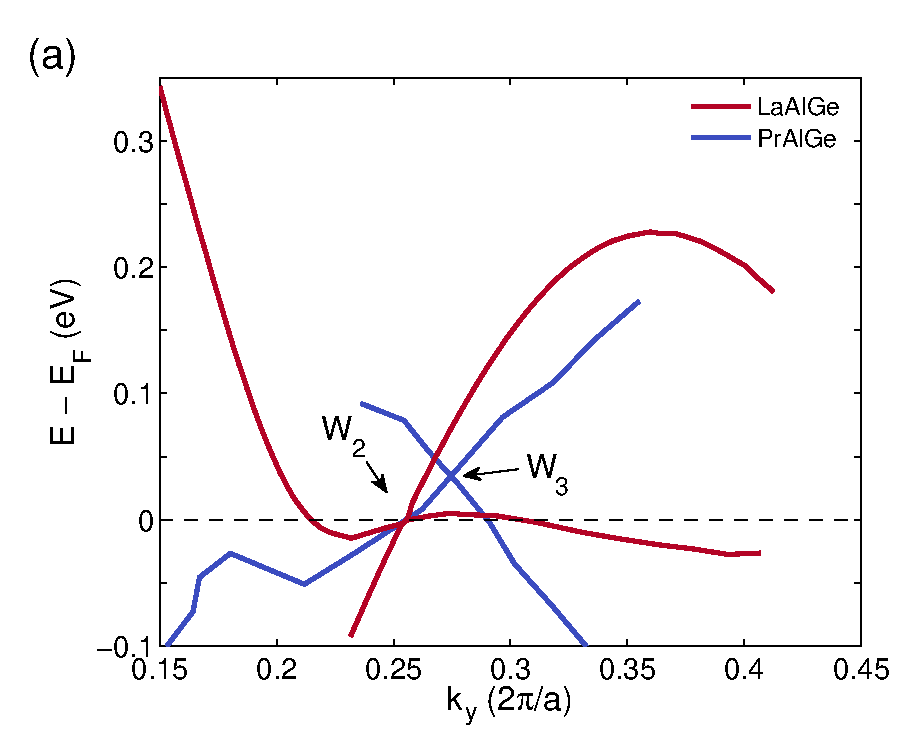
\includegraphics[width=0.320\textwidth,angle=0]{figures/PrAlGe/weylpoints}
	\hspace{5mm}
	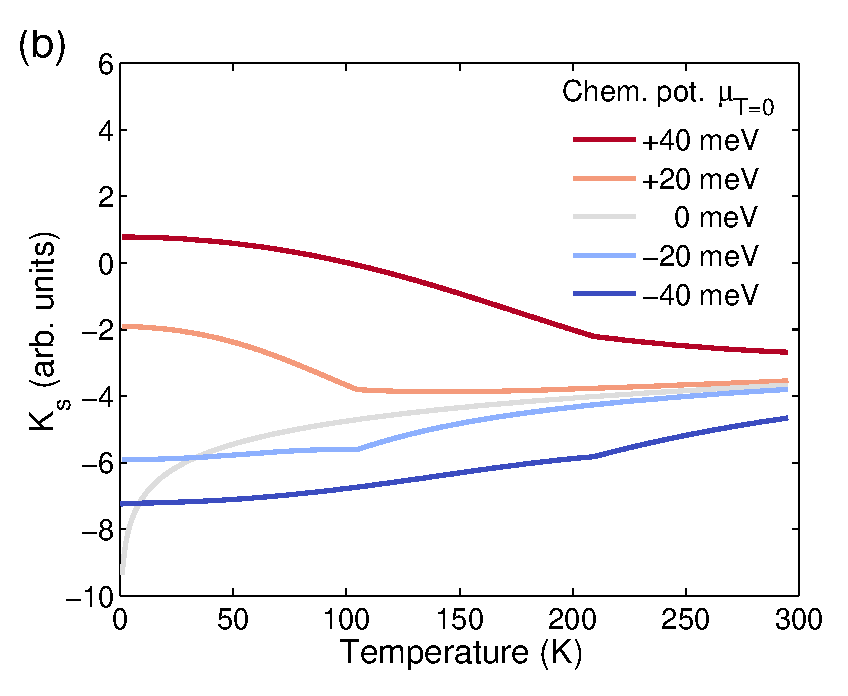
\includegraphics[width=0.312\textwidth,angle=0]{figures/PrAlGe/weylKS}
	%%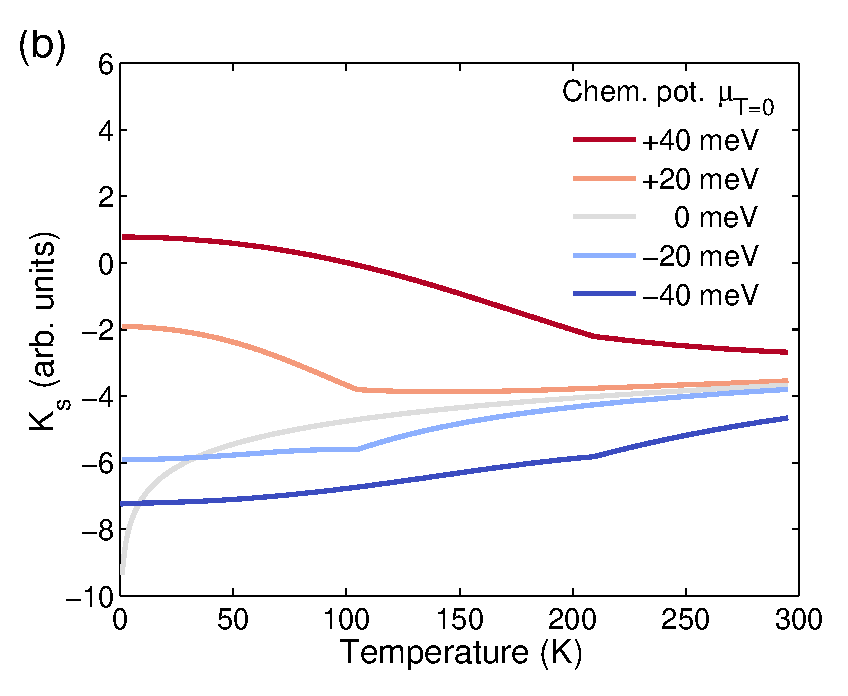
\includegraphics[width=0.4\textwidth,angle=0]{figures/PrAlGe/weylKS.eps}
	%\label{fig:weylKS}%\label{fig:PrAlGe_c_axis_7T_lines}
	%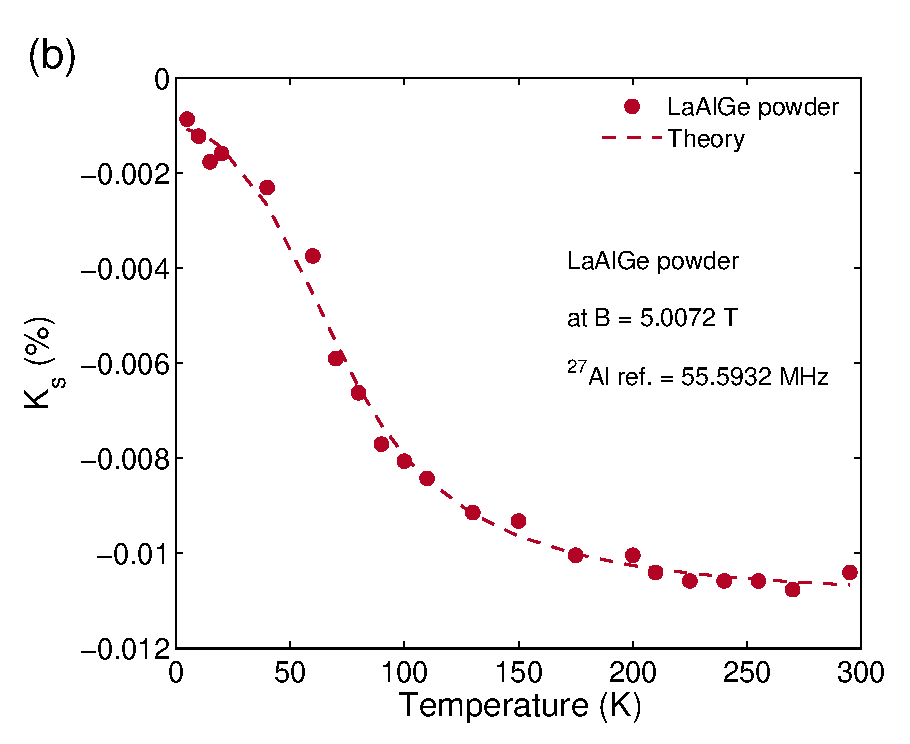
\includegraphics[width=0.32\textwidth,angle=0]{figures/LaAlGe_Powder/weylfit}%\%%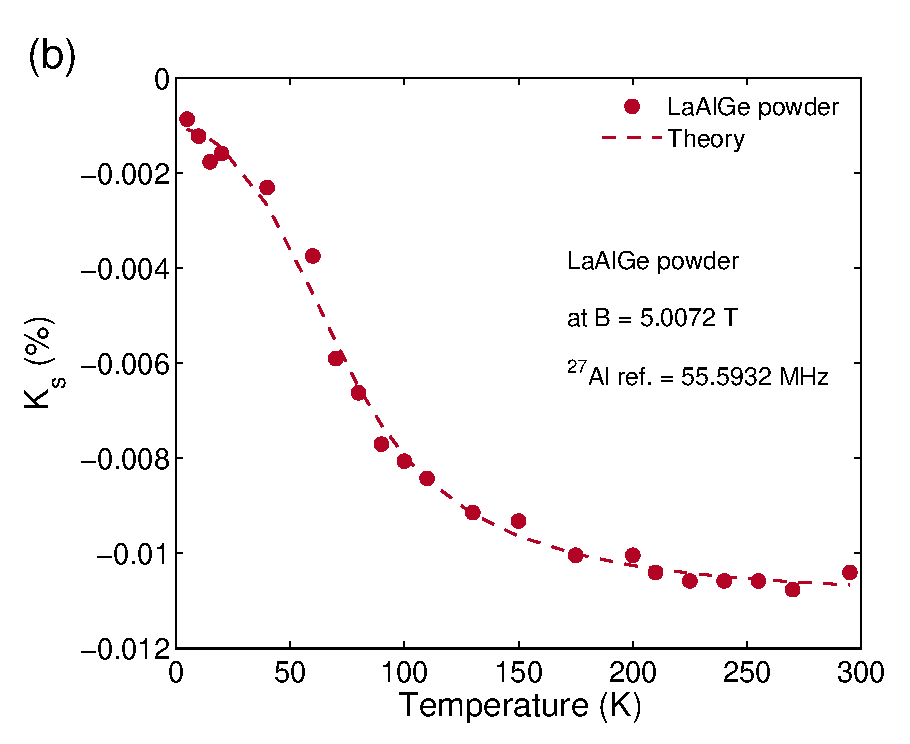
\includegraphics[width=0.4\textwidth,angle=0]{figures/LaAlGe_Powder/weylfit.eps}%\label{fig:PrAlGe_c_axis_7T_lines}
	\caption{\label{fig:weylKS}(a) Energy-momentum dispersion along the
	$k_{y}$ direction, as calculated from ARPES data for LaAlGe and
	PrAlGe \cite{xue2017discovery,sanchez2020observation}. 
	%The curves are calculated at different k_{x} and k_{z}.
	The arrows indicate the $W_2$ and $W_3$ Weyl nodes %in LaAlGe ($W_2$) and
	%PrAlGe ($W_3$)
	located in proximity of the Fermi level.
	(b) Knight shift vs temperature for typical values of the chemical potential \tcr{$\mu_{T=0}$}, as resulting from Eq.~\eqref{eqn:knightshiftmasterequation}. For convenience, we neglect the constant term and choose typical coefficients for the term proportional to $\mu$ and the logarithmic term, i.e., $K(\mu,T) = 100\mu + \ln\left(\max \left[|\mu|, k_\mathrm{B} T\right]\right)$. 
	The Knight-shift vs temperature for LaAlGe is shown in
	Fig.~\ref{fig:LaAlGe}(b).
	The fit to Eq.~\eqref{eqn:knightshiftmasterequation} %provides a
	gives \tcr{$\mu_{T=0} = 16.74$\,meV}, with $\mu = 0$ corresponding to the
	chemical potential of the Weyl point.
	}
	%Top: Temperature independent shift in metallic Al (blue line).}
\end{figure*}


For comparison, we show the same type of data obtained in an applied 
magnetic field of 7\,T. As in 5\,T, the same huge NMR shift of more 
than 10\,MHz persists [see Fig.~\ref{fig:PrAlGe_c_axis_5T}(b)], 
likewise accompanied by a large broadening of the NMR linewidth %of almost 3\,MHz
[see Fig.~\ref{fig:PrAlGe_c_axis_5T}(c)].
%
As exemplified in Figs.~\ref{fig:magnetometry}(a) and \ref{fig:magnetometry}(b),
both $\chi(T)$ and $K(T)$ are only weakly affected by the %a varying
external magnetic field. The Clogston-Jaccarino plot $K(\chi)$, involving data 
obtained at 5\,T, as displayed in Fig.~\ref{fig:magnetometry}(c), clearly
reveals that $K(T)$ is dominated by $\chi(T)$ also for this type of material.
Finally we note that $K(T)$ at both 5 and 7\,T is represented by a
Curie-Weiss-type fit with the same $\Theta_\mathrm{W}$ temperature of
31.7\,K. This value is practically identical to $\Theta_\mathrm{W} = 32$\,K,
calculated from fitting the magnetic susceptibility data $\chi(T)$ shown
in Fig.~\ref{fig:magnetometry}(a).

%The main difference between the NMR shifts at 5 and 7\,T appears in the temperature range between 16 and 30\,K where, as expected from the proximity to  $\Theta_\mathrm{W}$, the NMR shifts begin to diverge from the Curie-Weiss law. In this regime, as shown by the Clogston-Jaccarino plot in Fig.~\ref{fig:magnetometry}(c), (a relationship between macro- vs.\ microscopic magnetic susceptibility), the shifts in both 5 and 7\,T depend on the susceptibility in a nonlinear manner, but the shifts in 5\,T are consistently higher than those at 7\,T.
%\tcr{The enhanced nonlinearity in the 7-T case is not easy to pin down.
%Most probably, it reflects a yet unknown influence of the magnetic field
%on the Weyl states.}
%
%Finally, we note that the temperature dependence of the NMR shifts
%both in 5\,T and in 7\,T can be fit by a Curie-Weiss type law,
%with the same %Curie-Weiss
%\tcr{$\Theta_\mathrm{W}$ temperature of 31.7\,K}  
%[see Fig.~\ref{fig:magnetometry}(b)]. 
%Such %$\Theta_\mathrm{W}$
%value is close to $\Theta_\mathrm{W} = 32$\,K, calculated from
%the temperature dependence of the magnetic
%susceptibility $\chi(T)$ reported earlier \cite{sanchez2020observation}. 


%
%\begin{figure*}[!htb]
%	\centering 
%	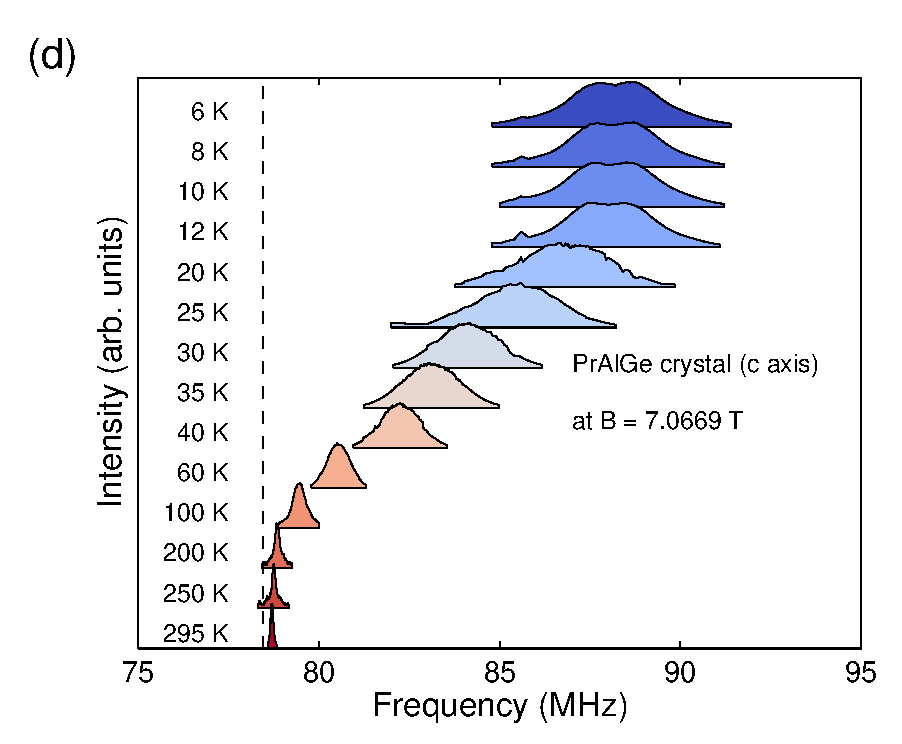
\includegraphics[width=0.32\textwidth,angle=0]{figures/PrAlGe_c_axis_7T/PrAlGe_c_axis_lines_vs_temp}%\label{fig:PrAlGe_c_axis_7T_lines}
%	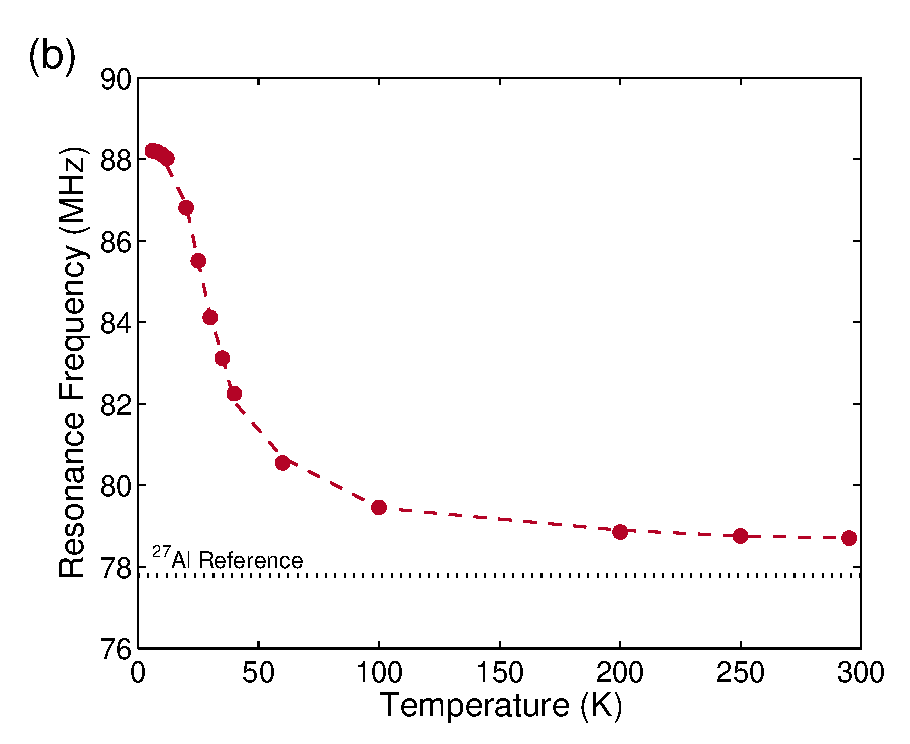
\includegraphics[width=0.32\textwidth]{figures/PrAlGe_c_axis_7T/gaussianshift.eps}%\label{fig:PrAlGe_c_axis_7T_shifts}
%	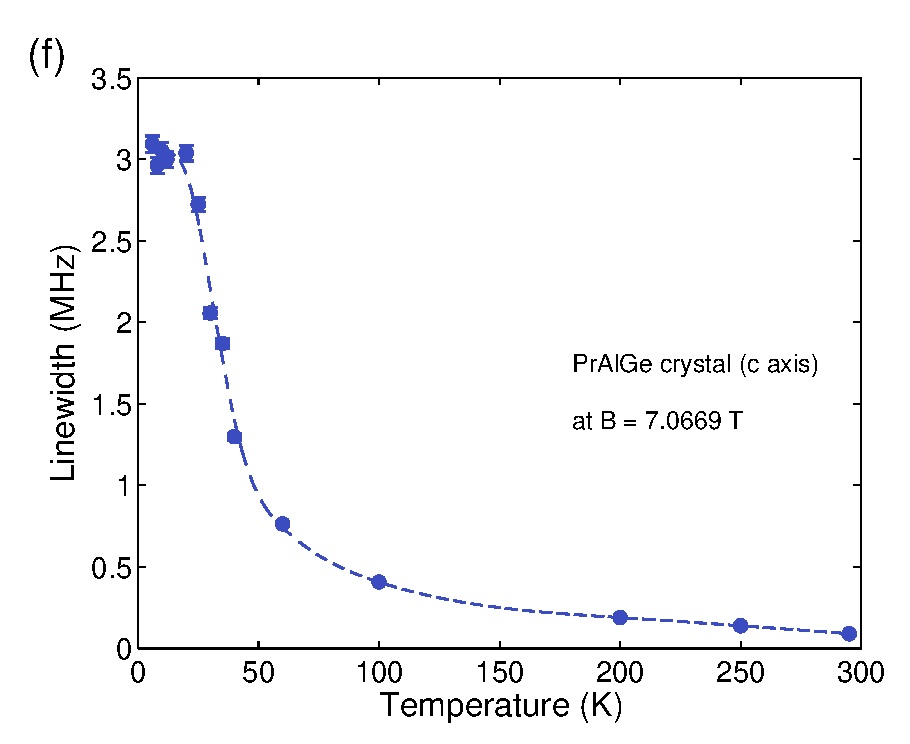
\includegraphics[width=0.33\textwidth]{figures/PrAlGe_c_axis_7T/gaussianwidth}%\label{fig:PrAlGe_c_axis_7T_widths}
%	\caption{\label{fig:PrAlGe_c_axis_7T}(a) Lineshapes (b) Lineshifts  and (c) Linewidths for $^{27}$Al NMR in magnetic PrAlGe crystal aligned along the $c$-axis measured in a 7-T external applied field. The black line indicates the position of reference Al NMR line %-- 1.1 m Al(NO$_{3}$)$_{3}$ in D$_{2}$O 
%	while the dashed lines are guides to the eye.}
%\end{figure*}
%



%\section{Discussion}
\emph{Discussion.---} 
Of prime interest here is a comparison of the experimental data of the 
$^{27}$Al NMR lineshift in LaAlGe with those measured in Al metal
\cite{bennett1970relevance} where, incidentally, $K(T) > 0$. As mentioned
in the caption of Fig.~\ref{fig:LaAlGe}(b), on the chosen scale, $K(T)$
in Al metal is represented by a horizontal line above %very close to
the baseline $K = 0\%$. This is indeed very different from the LaAlGe
dataset displayed in the same figure.

In order to interpret our lineshift data we employ the theory
%results presented
outlined in Refs.~\cite{okvatovity2016anomalous} and
\cite{Okvtovity2019nuclear}, where the anomalous hyperfine coupling of
nuclear spins in Weyl metals is discussed. The Hamiltonian describing
the spin-dipole part of the hyperfine coupling is identical for common-
and Weyl metals. The essential difference is that between the orbital parts.
In ordinary metals, the orbital component of the electronic susceptibility
describes the interaction between the nuclear spins and the orbital
motion of electrons [see Eq.~\eqref{eqn:HFI_metal}]. In the case of Weyl fermions,
instead, the orbital term is replaced by the spin of the Weyl quasiparticles
[here denoted by the Pauli matrices $\sigma=(\sigma_{x},\sigma_{y},\sigma_{z}$)]. 
According to Ref.~\cite{okvatovity2016anomalous}, the respective
interactions are given by:
%
%In ordinary metals, the orbital component of the electronic susceptibility 
%describes the interaction between nuclear spins and the orbital motion 
%of electrons [see Eq.~\eqref{eqn:HFI_metal}]. In the case of Weyl fermions, 
%instead, the orbital term %still contains 
%is replaced by the spin of the Weyl quasiparticles [here denoted by the 
%Pauli matrices $\sigma=(\sigma_{x},\sigma_{y},\sigma_{z}$)]. Thus, for 
%Weyl fermions, the hyperfine electron-nucleus interaction ends up being 
%a spin-spin interaction [see Eq.~\eqref{eqn:HFI_weyl}] \cite{okvatovity2016anomalous}:
%
\begin{align}
\mathscr{H}_{\mathrm{HFI}}^{\mathrm{orb}} &= \frac{\mu_{0}}{4 \pi} \hbar \gamma_{\mathrm{n}} g \mu^{*} \, \boldsymbol{I} \frac{\boldsymbol{r} \times \boldsymbol{p}}{\hbar r^{3}} \qquad \text{for free electrons,} \label{eqn:HFI_metal} \\[3mm]
%
\mathscr{H}_{\mathrm{HFI}}^{\mathrm{orb}} &= \frac{\mu_{0}}{4 \pi} \hbar \gamma_{\mathrm{n}} e v_{\mathrm{F}} \, \boldsymbol{I} \frac{\boldsymbol{r} \times \boldsymbol{\sigma}}{r^{3}} \qquad \text{for Weyl fermions.}
\label{eqn:HFI_weyl}
\end{align}

%
%\begin{equation}
%H_{\mathrm{HFI}}^{\mathrm{orb}}=\frac{\mu_{0}}{4 \pi} \hbar \gamma_{\mathrm{n}} g \mu^{*} \mathbf{I} \frac{\mathbf{r} \times \mathbf{p}}{\hbar r^{3}} \qquad \text{for free electrons,}
%\label{eqn:HFI_metal}
%\end{equation}
%
%\begin{equation}
%H_{\mathrm{HFI}}^{\mathrm{orb}}=\frac{\mu_{0}}{4 \pi} \hbar \gamma_{\mathrm{n}} e v_{\mathrm{F}} \mathbf{I} \frac{\mathbf{r} \times \boldsymbol{\sigma}}{r^{3}} \qquad \text{for Weyl fermions.}
%\label{eqn:HFI_weyl}
%\end{equation}

\noindent
Here, $v_\mathrm{F}$ is the Fermi velocity, $\mu^{*}$ is the 
renormalized chemical potential, $g$ the electron $g$-factor,  % density of states at the Fermi level, 
and $\mu_{0}$, $\hbar$, $k_\mathrm{B}$, $e$ are physical constants.

In ordinary metals, the orbital component $H_{\mathrm{HFI}}^{\mathrm{orb}}$ is usually assumed to be temperature independent and thus included in the temperature-independent NMR shift $K_{0}$. 
In Weyl semimetals, instead, $H_{\mathrm{HFI}}^{\mathrm{orb}}$ has an implicit temperature dependence due to $\sigma$, which is related to the temperature-dependent susceptibility. Consequently, in Weyl semimetals, 
we can decompose the Hamiltonian into a tem\-pe\-ra\-ture\--independent 
and a temperature-dependent part: $\mathscr{H} = \mathscr{H}_{0} + \mathscr{H}^{\prime}(T)$. 
%with $\mathscr{H}^{\prime}(T)$ 
%refers to the temperature-dependent part.
After some calculations 
\cite{Okvtovity2019nuclear}, $\mathscr{H}^{\prime}(T)$ can be expressed as: 
%
\begin{equation}
\mathscr{H}^{\prime}(T)=e v_\mathrm{F}\, \boldsymbol{\sigma}(T) \cdot \boldsymbol{A} 
+ \frac{g \mu_{B}}{2} \, \boldsymbol{\sigma}(T) \cdot \boldsymbol{B}, 
\label{eqn:externalfield}
\end{equation}
%
where $\boldsymbol{A}$ denotes the magnetic vector potential and $\boldsymbol{B}$  
the magnetic field. Note that, besides the usual Zeeman energy term, 
proportional to $\boldsymbol{\sigma}(T) \cdot \boldsymbol{B}$, there is 
also an additional term, proportional to $\boldsymbol{\sigma}(T) \cdot \boldsymbol{A}$. 
After some algebraic manipulation, the temperature-dependent NMR shift 
due to the Weyl fermions can be expressed as \cite{Okvtovity2019nuclear}: 
% (Eq.~\eqref{eqn:knightshiftmasterequation}).
%
\begin{equation}
K(\mu, T) \approx \frac{\mu_{0} e}{4 \pi^{2} \hbar}\left[\frac{g \mu_\mathrm{B}}{\hbar v_\mathrm{F}} \mu - \frac{e v_\mathrm{F}}{3} \ln \left(\frac{W}{\max \left[|\mu|, k_\mathrm{B} T\right]}\right)\right].
\label{eqn:knightshiftmasterequation}
\end{equation}
%
%
\begin{figure*}[!thb]
	%\centering
	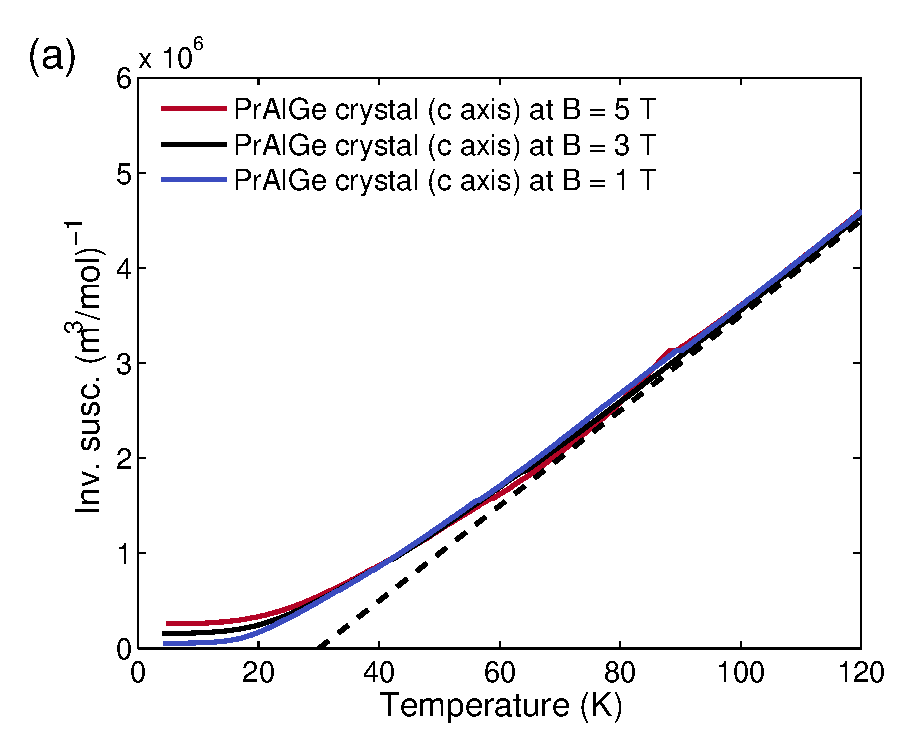
\includegraphics[width=0.32\textwidth,angle=0]{figures/PrAlGe/invsusceptibilityvsT.eps}%\label{fig:PrAlGe_c_axis_7T_lines}
	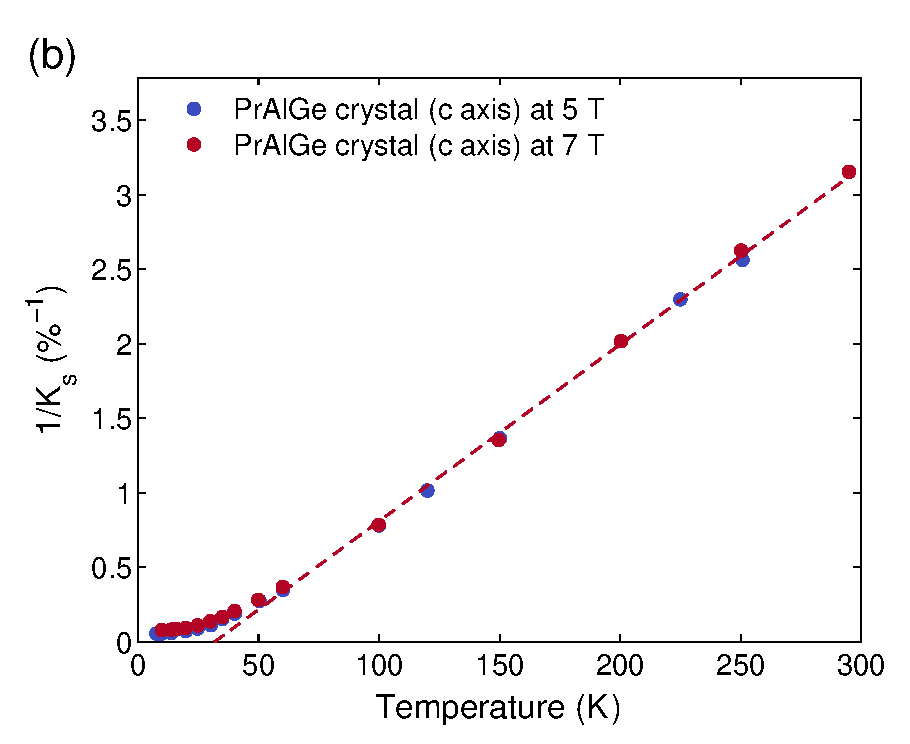
\includegraphics[width=0.32\textwidth]{figures/PrAlGe/27AlinvS_vs_T}%\label{fig:CW}
	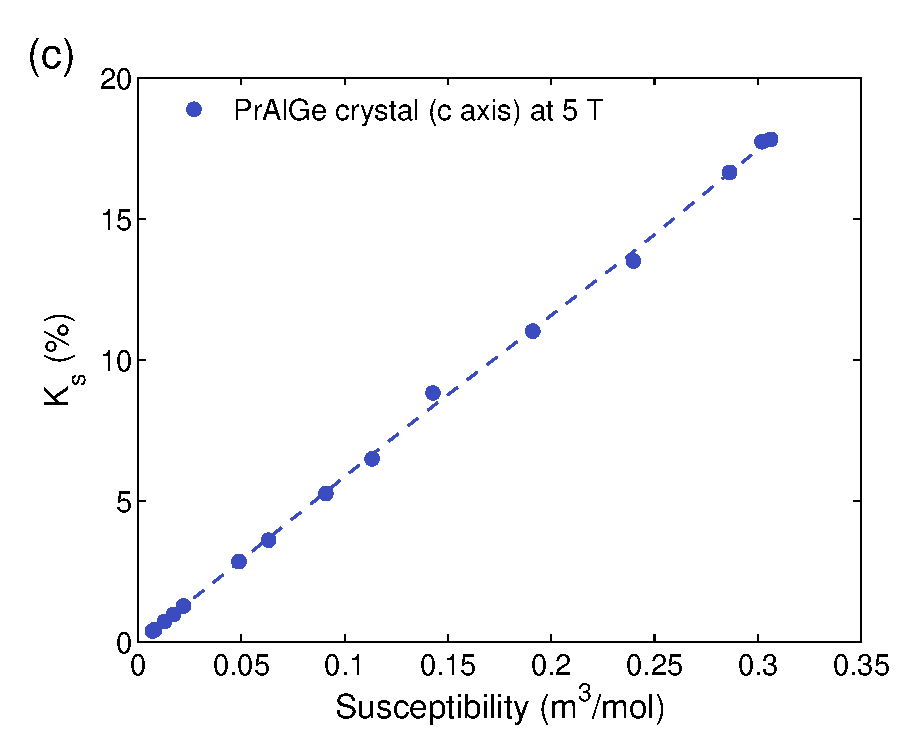
\includegraphics[width=0.32\textwidth]{figures/PrAlGe/27AlCJ_plot}%\label{fig:CJ}
    \caption{\label{fig:magnetometry}(a) Inverse susceptibility-, (b)
    Curie-Weiss-type $K_s(T)$, and (c) Clogston-Jaccarino plots
    showing the NMR shifts in a PrAlGe single crystal (with the field
    applied along the $c$-axis) vs temperature and magnetic
    susceptibility, respectively, as measured at 5\,T. 
    Note the coinciding datasets in panels (a) and (b) under
    different applied magnetic fields and the similar
    $\Theta_\mathrm{W}\sim 32$\,K values ($T$-axis intercepts). 
    The dashed lines in (a) and (b) represent fits to the 
    Curie-Weiss law. The fit in (c) highlights the linear 
    relationship between the magnetic susceptibility and NMR line shift.}
    %\tcr{Note the coinciding inverse susceptibility data in panel (a)
    %and inverse shifts in panel (b) under different applied magnetic fields.}.}
\end{figure*}
%
%corresponds to the Clogston-Jaccarino theory, which posits a 
%linear relationship between magnetic susceptibility and NMR shift.
%. In panels A and B, 
%the lines correspond to an inverse Curie-Weiss fit, hence showing that 
%the inverse shift is proportional to temperature. In panel C, the linear 
%fit corresponds to the Clogston-Jaccarino theory, which posits a 
%linear relationship between magnetic susceptibility and NMR shift. 
%
%
Here, $W\gg\mu$ is a sharp high-energy cutoff 
regularizing the theory, while $\mu$ denotes the chemical potential away 
from the Weyl point. Note that $\mu$ contains an implicit 
temperature dependence (see Ref.~\cite{Okvtovity2019nuclear} for details). 
The most salient feature of Eq.~\eqref{eqn:knightshiftmasterequation} is 
that at high temperatures \tcr{($k_\mathrm{B}T\gg\mu$)}, the Knight shift $K$ is dominated 
by the $-\ln(W/k_\mathrm{B}T)$ term, which gives rise to 
a \emph{negative shift} \tcr{regardless of the $\mu$} value. 

%\begin{figure}[!htb]
%	\centering 
%	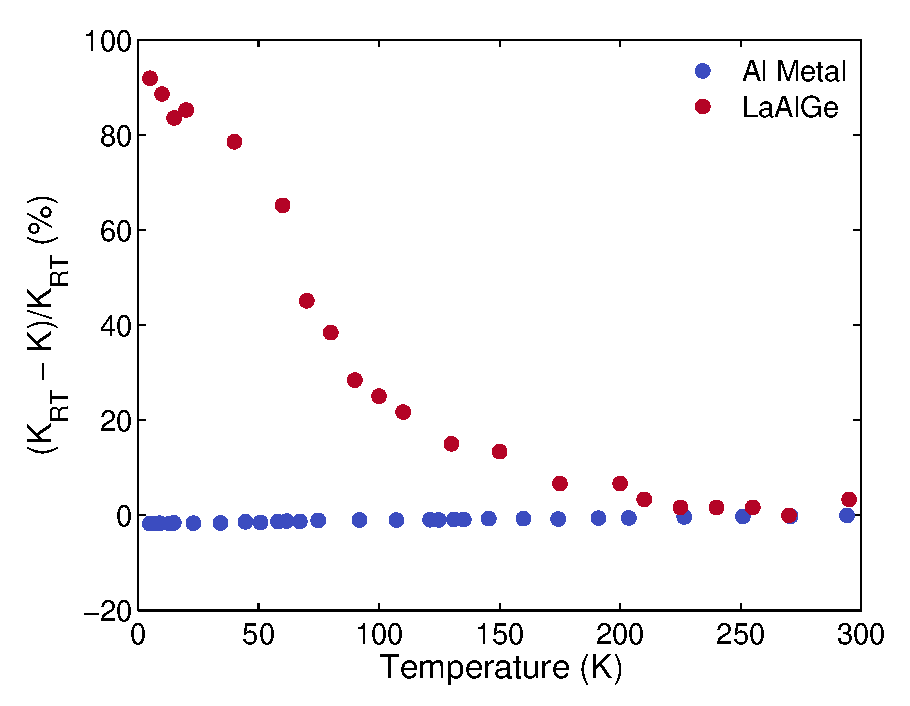
\includegraphics[width=0.4\textwidth,angle=0]{figures/LaAlGe_Powder/LaAlGe_powder_vs_Al_metal_shift_change.eps}%\label{fig:PrAlGe_c_axis_7T_lines}
%	\caption{\label{fig:LaAlGevsAl} Change in NMR Shift vs Temperature, normalized to the NMR shift at room Temperature. In contrast metallic ${^27}$Al, where the NMR shift shows a weak temperature dependence, the NMR shift in LaAlGe changes significantly with temperature. }
%\end{figure}
%
%
%\begin{figure}[!htb]
%	\centering 
%	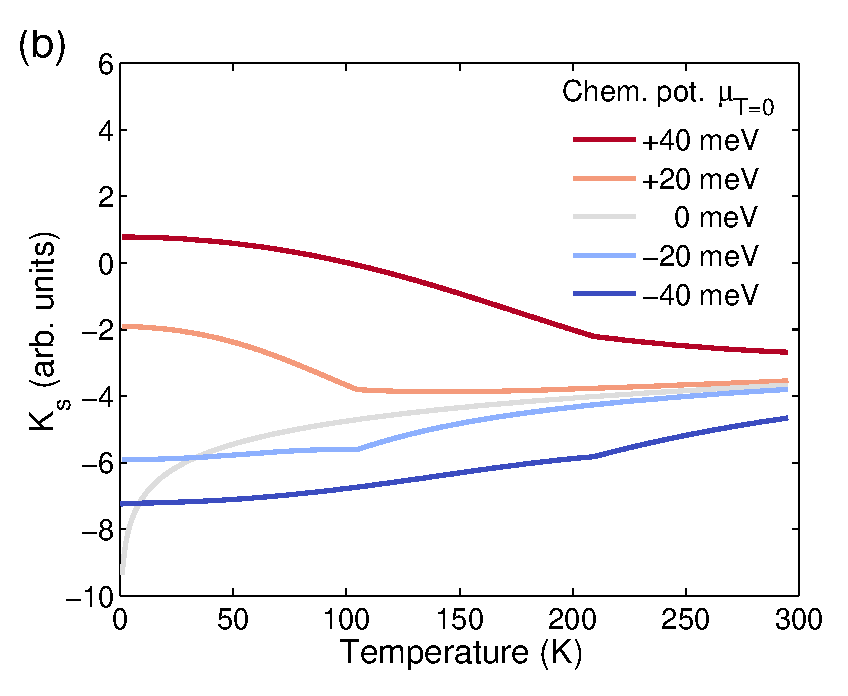
\includegraphics[width=0.4\textwidth,angle=0]{figures/PrAlGe/weylKS.eps}%\label{fig:PrAlGe_c_axis_7T_lines}
%	\caption{\label{fig:weylKS}Knight shift dependence vs temperature for typical values of the chemical potential $\mu(T=0)$, as resulting from Eq.~\eqref{eqn:knightshiftmasterequation}. For convenience, we neglect the constant term and choose typical coefficients for the term proportional to $\mu$ and the the logarithmic term, i.e., $K(\mu,T) = 100\mu + \ln\left(\max \left[|\mu|, k_\mathrm{B} T\right]\right)$.}
%\end{figure}

%\begin{figure}[!htb]
%	\centering 
%	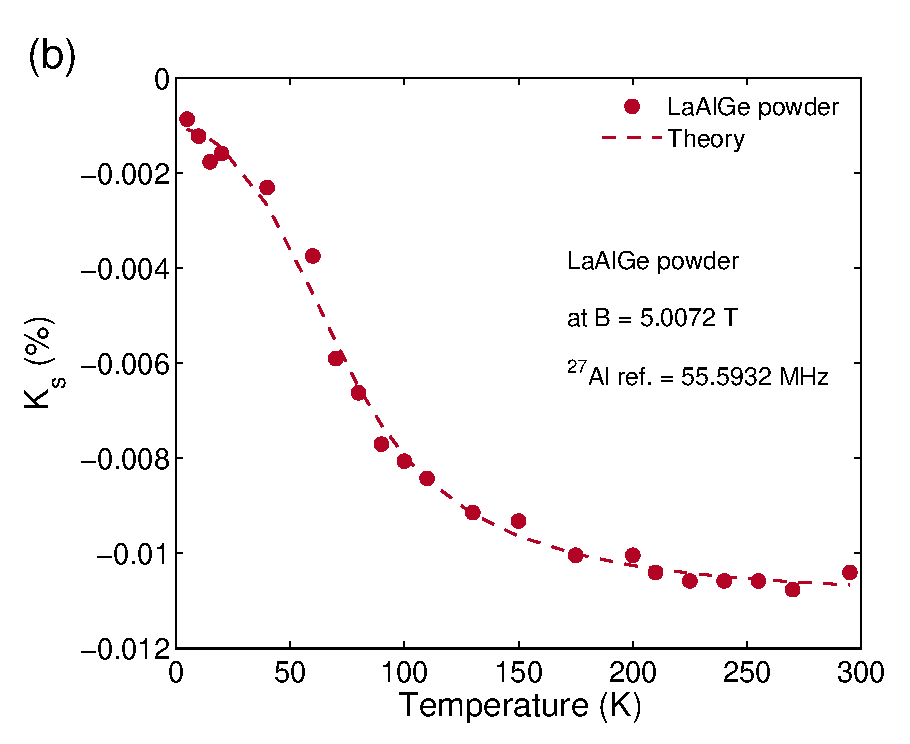
\includegraphics[width=0.4\textwidth,angle=0]{figures/LaAlGe_Powder/weylfit.eps}%\label{fig:PrAlGe_c_axis_7T_lines}
%	\caption{\label{fig:weylfit}Knight shift dependence vs temperature for LaAlGe, fit to Eq. \ref{eqn:knightshiftmasterequation}. The calculated value of $\mu$ is $16.74$ meV}
%\end{figure}

The NMR shifts in LaAlGe can be explained qualitatively by this theory. 
From Fig.~\ref{fig:LaAlGe}(b), %Fig.~\ref{fig:weylKS}(c),
it is clear that $K_s(T)$ in LaAlGe,
although small, is \emph{qualitatively different} from the
free-electron type $K_s(T)$ in the Al metal \cite{bennett1970relevance}.
Therefore, we propose that the observed NMR shifts in LaAlGe are indeed
due to the Weyl node features.  

Based on ARPES measurement results \cite{xue2017discovery}, it was
concluded that LaAlGe exhibits three classes of Weyl nodes, denoted by $W_1$, $W_2$, and 
$W_3$ respectively. The $W_2$ nodes are type-II Weyl nodes, whereas the 
$W_1$, $W_3'$, and $W_3''$ nodes are of type-I. %The main difference between them consists in
In particular, the $W_2$ Weyl nodes are located almost exactly at the
Fermi level [see Fig.~\ref{fig:weylKS}(a)], whereas the $W_1$, $W_3'$, and $W_3''$ Weyl nodes are about 60, 110, and 130 meV above the Fermi level, respectively. Considering the very low energies involved in a typical NMR experiment 
(about tens of $\mu$eV), we may assume that the NMR response is due exclusively to the $W_2$ nodes. 

\tcr{NMR shifts due to a Weyl node in the typical $\pm 40$\,meV 
range are illustrated in Fig.~\ref{fig:weylKS}b, where we plot Eq.~\eqref{eqn:knightshiftmasterequation} 
for selected values of $\mu_{T=0}$. We note that the shift at room temperatures is typically  \emph{negative}.} As the temperature decreases, the NMR shift is increasingly dominated by $\mu$ and hence, as expected from Eq.~\eqref{eqn:knightshiftmasterequation}, 
it becomes less negative. 
Due to the implicit temperature dependence 
of $\mu$, at intermediate $T$ values, the Knight shift vs temperature curves 
change with varying $\mu_{T=0}$. Nevertheless, %the common feature is that 
the typical Knight shifts at a single Weyl node are predominantly negative, 
%: In our simple model, the Knight shifts only 
%to become
turning positive only at unphysically large $\mu_{T=0}$ values. 
In LaAlGe, in particular, a fit with \tcr{$\mu_{T=0}=+16.74$\,meV} provides a fairly 
good agreement between the experiment and theory
[see Fig.~\ref{fig:LaAlGe}(b)]. 
%[see Fig.~\ref{fig:weylKS}(c)]. 
%(see Fig.~\ref{fig:weylfit}). 
\tcr{Given the relatively high chemical potential 
of $+16.74$\,meV, the Fermi surface is rather far from the Weyl 
point. The satisfactory fit by means of Eq.~\eqref{eqn:knightshiftmasterequation} 
suggests that, under these circumstances, the system is less sensitive to 
the details of the dispersion relation near the Weyl point. At the 
current level of experimental precision, we do not observe any additional 
effects arising from the type-II classification of the Weyl node in LaAlGe.}



%\begin{figure}[!htb]
%	\centering 
%	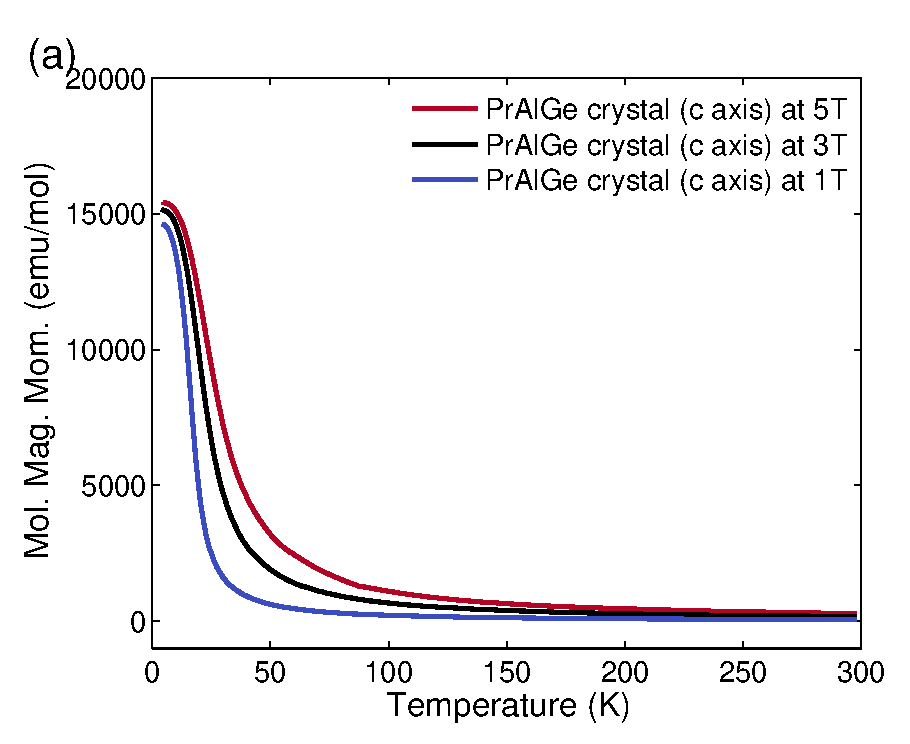
\includegraphics[width=0.4\textwidth,angle=0]{figures/PrAlGe/magmovsT.eps}\\%\label{fig:PrAlGe_c_axis_7T_lines}
%	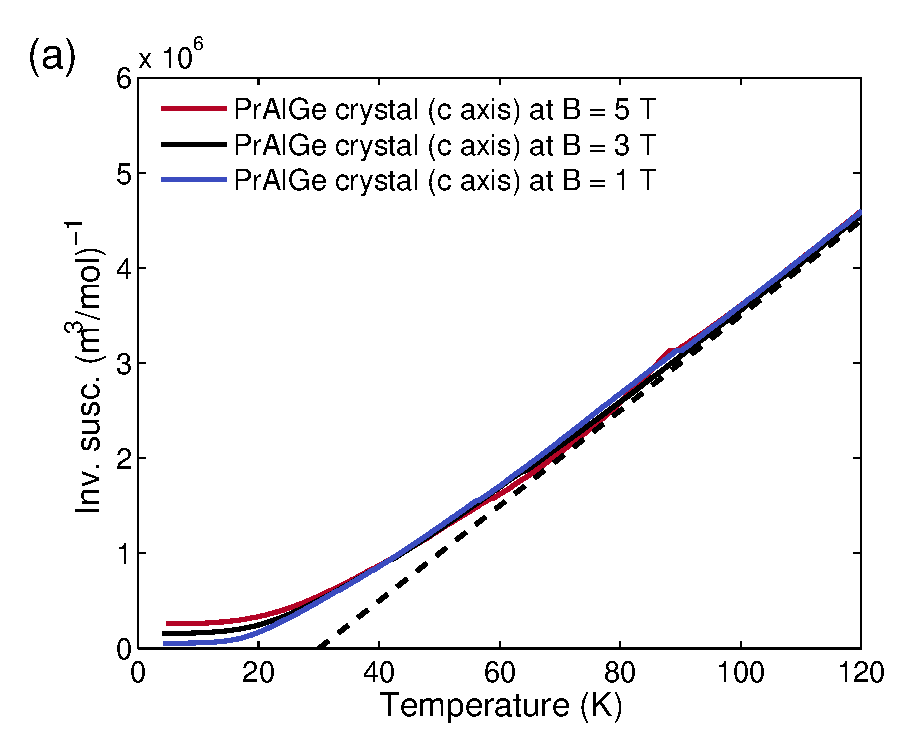
\includegraphics[width=0.4\textwidth,angle=0]{figures/PrAlGe/invsusceptibilityvsT.eps}%\label{fig:PrAlGe_c_axis_7T_lines}
%	\caption{\label{fig:magnetometry} (a)  Magnetic Moment and (b) Inverse Susceptibility of PrAlGe.  In contrast to PrAlGe, which exhibits a strong ferromagnetic response with $\Theta_{W}\approx32$\,K, LaAlGe does not exhibit any significant magnetic response when plotted against the same scale }
%\end{figure}
%









%\begin{figure}[!thb]
	%\centering
%	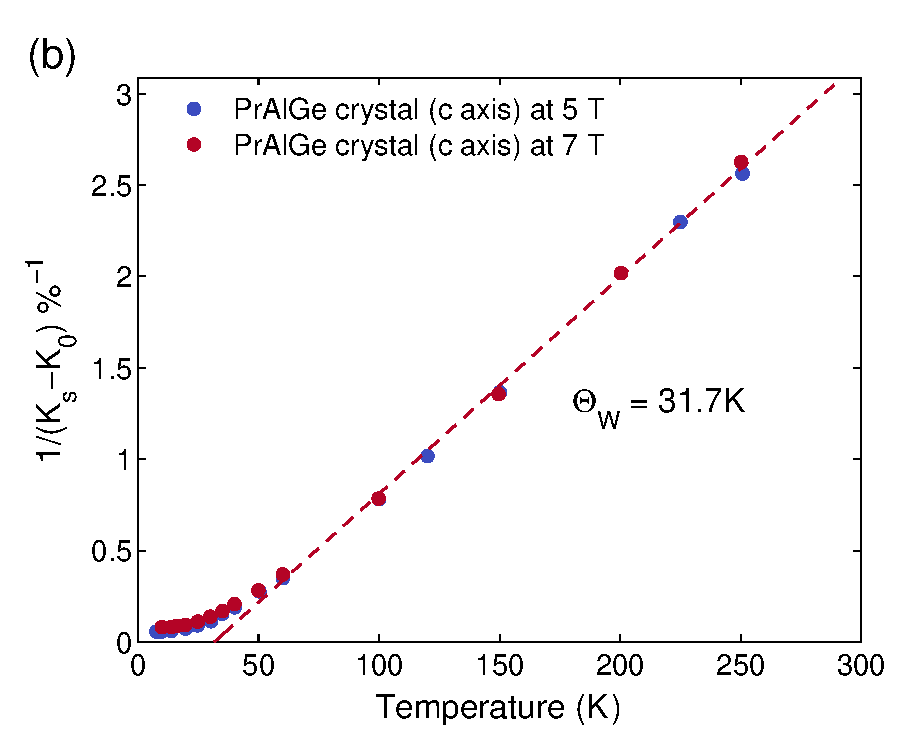
\includegraphics[width=0.4\textwidth]{figures/PrAlGe/27AlinvKS_vs_T}\\%\label{fig:CW}
%	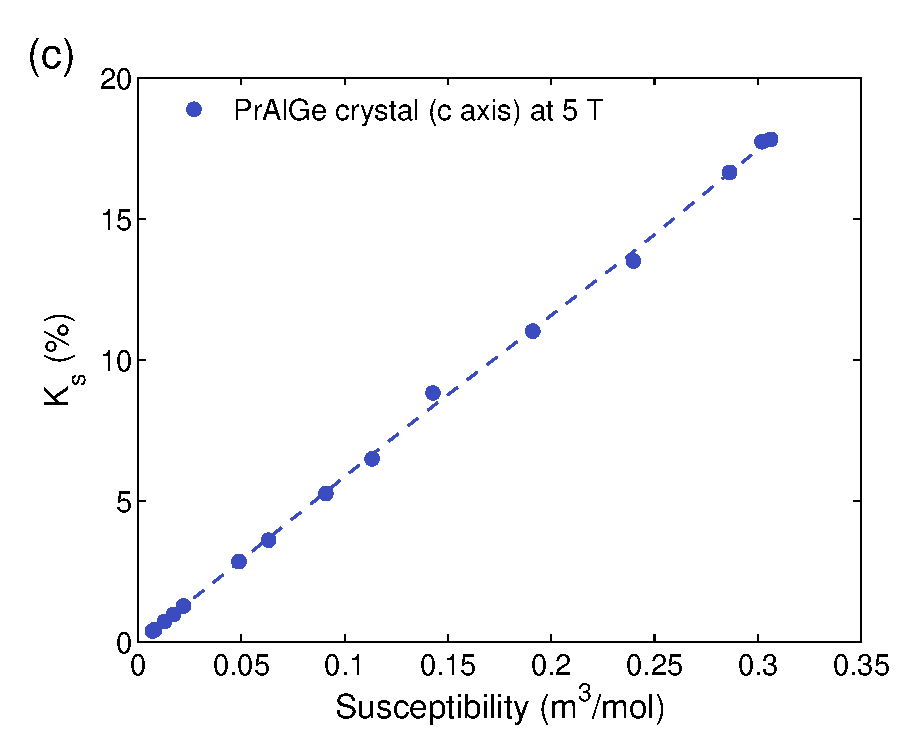
\includegraphics[width=0.4\textwidth]{figures/PrAlGe/27AlCJ_plot}%\label{fig:CJ}
%   \caption{\label{fig:CWCJ}Curie-Weiss- (a) and Clogston-Jaccarino plot (b) showing the NMR 
%    shifts of a PrAlGe crystal ($c$-axis) vs temperature and magnetic susceptibility, respectively, measured at 5 and 7\,T.  }
%\end{figure}

On the other hand, in PrAlGe, the giant NMR shift cannot be accounted for by Eq.~\eqref{eqn:knightshiftmasterequation} only. 
While it is certain that Weyl nodes exist also in PrAlGe --- theoretical models \cite{chang2018magnetic} and ARPES results %measurement data 
\cite{sanchez2020observation} agree that there are at least two ($W_3$ and $W_4$) Weyl nodes within +20\,meV from the Fermi surface [Fig.~\ref{fig:weylKS}(a)] ---
the giant NMR shift we observe in PrAlGe is \emph{orders of magnitude}
larger than the $\sim 0.1\%$ shifts observed in most Weyl systems studied
so far (see, e.g., Ref.~\cite{antonenko2019nmr,Okvtovity2019nuclear,Wang2020landau}).
Clearly, the character of those shifts is qualitatively
different from that observed in PrAlGe. %in the other Weyl systems.
The dominant contribution to Eq.~\eqref{eqn:knightshiftmasterequation}
is the negative logarithmic term, which is \emph{opposite} in sign to
the NMR shift observed in PrAlGe. The fact that the shifts at 5 and 7\,T
follow the same temperature dependence above the Curie temperature
[see Fig.~\ref{fig:magnetometry}(b)], rules out the splitting of
energy bands due to Landau diamagnetism \cite{Wang2020landau}.

As shown in Fig.~\ref{fig:magnetometry}(a), PrAlGe exhibits the typical
$\chi(T)$ features of rare-earth compounds with $4f$-electron local
moments on regular lattice sites. On the other hand, our $\chi(T)$ data
for LaAlGe indicate a weak diamagnetic response across the entire
covered temperature range. %(not shown, since it is too trivial).
Therefore, the $^{27}$Al NMR resonance shift $K(T)$ in PrAlGe is expected
to be dominated by the transferred hyperfine field
\cite{dunlap1972orbital,jones1969nuclear} due to %the presence of
the Pr$^{3+}$ ions. At elevated temperatures and at different applied
magnetic fields, this contribution overshadows %obfuscates masks
a possible influence of the Weyl-type quasiparticles on $\chi(T)$.

%\tcb{This statement is wrong! Even though, the moments are local, does not mean that the field can not influence the $\chi{T}$. For example, in the magnetic order state, many rare-earth sample show metamagentic transition under field. If you only refer to the PM state, it should be clearly written.}



As mentioned above, the close connection between $K(T)$ [see Fig.~\ref{fig:magnetometry}(b)]
and $\chi(T)$ is confirmed by the Clogston-Jaccarino type plot shown in
Fig.~\ref{fig:magnetometry}(c), where data recorded in a magnetic field
of 5\,T are shown as an example.
%
%We propose that the giant NMR shift in PrAlGe can be explained by adding to the expression for the $K(\mu,T)$ NMR shift an additional term that describes the transferred hyperfine coupling field due to the Pr$^{3+}$ ions. Indeed, it is known that in rare-earth metals, the conduction $s$ electrons couple with the $4f$ electrons via the $s$-$f$ exchange interaction, which polarizes the conduction electrons and gives rise to a transferred hyperfine field \cite{dunlap1972orbital,jones1969nuclear}. In this case, the resulting total shift %that results from this transferred hyperfine field can be expressed as \cite{feller198227Al}:
%
%\begin{equation}
%\label{eqn:hyperfineknightshift}
%K = K_0 + K_f = K_0 \left[1 - J_{sf} \frac{g_J - 1}{g_J \mu_{\mathrm{B}}^{2}} \, \frac{\chi_{f}^{0}}{N_{f}}\right] = K_0 \left(1+\lambda_{sj} \chi_{f}^{0}\right),
%\end{equation}
%
%where $K_0$ denotes the usual paramagnetic contribution of the conduction electrons, 
%while $K_{f}$ denotes the additional shift due to the transferred hyperfine fields. 
%
The magnitude of the NMR shifts that we obtain in PrAlGe is consistent with the 
typical magnitudes of NMR shifts in compounds known to possess transferred hyperfine fields. 
%In the existing literature, 
Typical values of the transferred hyperfine field in Pr compounds 
are in the range 1.3 to 13.6\,T \cite{dunlap1972orbital,jones1969nuclear}, 
thus giving rise to correspondingly large NMR shifts. For instance, PrP
shows a maximum NMR shift of 12\% \cite{jones1969nuclear},
while PrAl$_{2}$ exhibits an even higher NMR shift of 17.5\% \cite{feller198227Al}.
This implies that the very large shifts observed in our case are
not a typical feature of Weyl-type metals, but rather a consequence of
the local-moment transferred hyperfine interactions with the itinerant
quasiparticles. As such, they appear to be similar in either conventional
metals or in Weyl-type semimetals.

%In general, the qualitative behavior of the NMR shifts we observe in PrAlGe 
%is consistent with the theory of transferred hyperfine fields. 
%Magnetometry measurements [Fig.~\ref{fig:magnetometry}(a)] show that 
%PrAlGe is strongly magnetic with a $\Theta_\mathrm{W}$ of approximately 30\,K. 
%Both the inverse Curie-Weiss [Fig.~\ref{fig:magnetometry}(a)] and the Clogston-Jaccarino 
%plots [Fig.~\ref{fig:magnetometry}(c)] show a linear dependence. Furthermore, the giant NMR 
%shifts are accompanied by a significant line broadening [see Fig.~\ref{fig:PrAlGe_c_axis_5T}(c) 
%and \ref{fig:PrAlGe_c_axis_5T}(f)], while such giant shifts are missing 
%in nonmagnetic LaAlGe [see Fig.~\ref{fig:LaAlGe}(a)].

%Although the NMR shift in PrAlGe is mostly due to the transferred 
%hyperfine field from the Pr$^{3+}$ ions, its exact mechanism cannot be 
%explained by the current state of theory [see Eq.~\eqref{eqn:hyperfineknightshift}], 
%since the latter 
%does not take the Weyl fermions into account. On the other hand, the current 
%theory of NMR shifts at Weyl nodes [see Eq.~\eqref{eqn:knightshiftmasterequation}] 
%does not take the transferred hyperfine fields into account. Therefore, it is clear 
%that to properly account for the giant NMR shift in PrAlGe, one %would have 
%needs to combine the above two contributions 
%(the Weyl-fermion and the transferred hyperfine) to the NMR shift, 
%a task beyond the scope of the current paper.



In conclusion, we presented a comparative $^{27}$Al NMR study of the
Weyl semimetal systems LaAlGe and PrAlGe. The NMR shifts in
LaAlGe can be described by an anomalous hyperfine coupling near the Weyl
point. On the other hand, the magnetic PrAlGe exhibits a giant NMR shift
of up to $20\%$ at 5\,T, which is absent in nonmagnetic LaAlGe.
Thus, in order to identify the typical features of Weyl-type semimetals,
the presence of local moments on the regular lattice sites of a chosen
material should be avoided.

%The giant NMR shift we observe cannot be explained by either the simplified model of a single Weyl point near the Fermi level or a band splitting due to Landau effects. Most likely, the large NMR shift is due to the interplay between the transferred hyperfine fields and Weyl nodes, which goes beyond the currently established theory of NMR in Weyl semimetals. More work is required to develop such a theory, which is expected to explain the huge NMR shifts reported here. 
%





%\subsection{Data availability.} 
%\footnotesize{%
%All the data needed to evaluate the reported conclusions 
%are presented in the paper and/or in the Supplementary Materials. Additional data
%related to this paper may be requested from the authors. The NMR data
%were generated at ETH Zurich (Zurich, Switzerland).
%Derived data supporting the results of this study are available from the %corresponding authors. 
%}

%\section{Acknowledgments}
%
%\emph{Acknowledgments.---}
We thank A.\ Grushin and S.\ Tsirkin for preliminary discussions
%on the electronic properties of PrAlGe
and C.\ Wang for assistance with the magnetometry measurements.
This work was supported by the 
Schwei\-ze\-rische Na\-ti\-o\-nal\-fonds zur F\"{o}r\-de\-rung der 
Wis\-sen\-schaft\-lich\-en For\-schung (SNF) via grants no.\ 
200021-169455 and 200021-188706.

%\section{Author contributions}
%\footnotesize{%
%T.S and P.P did the sample synthesis and susceptibility measurements.
%D.T, T.Sh. did the NMR samples
%D.T and T.Sh. wrote the paper with input from all the authors.
%}

%\section{Competing interests}
%\footnotesize{%
%The authors declare no competing financial interests.
%}

%\section{Additional information}
%\footnotesize{%
%\textbf{Supplementary Information} accompanies this paper at http://www.nature.com/naturecommunications.
%}


%\section{Figure legends}

%\begin{description}
%        \item[First] \hfill \ The first item
%
%\item[Fig.~\ref{fig:phase_diagram}] %1
%
%
%\item[Fig.~\ref{fig:ZF-MuSR}] %2
%
%
%\item[Fig.~\ref{fig:TF-MuSR}] %3
%
%
%\item[Fig.~\ref{fig:lambda}] %4
%
%
%
%
%\end{description}



\vspace{-5mm}

\renewcommand*{\bibfont}{\footnotesize}
%\begin{thebibliography}{99}
%\bibliographystyle{apsrev4-2}
\bibliography{PrAlGe_bib}
%\end{thebibliography}

%To get rid of bibtex jnrlst warning in Overleaf, insert in outputNotes.bib the following two lines:
%@CONTROL{REVTEX42Control}
%@CONTROL{apsrev42Control,author="48",editor="1",pages="0",title="",year="1"}
%See also, http://ipfs-sec.stackexchange.cloudflare-ipfs.com/tex/A/question/76028.html


% After running bibtex, copy the contents of the .bbl file into the original document.
% Comment the lines \bibliography{PrAlGe_bib} and \end{document} right here. 

\end{document}


